\documentclass[12pt]{article}

\usepackage[margin=1in]{geometry}
\usepackage{graphicx}
\usepackage{float}
\usepackage{hyperref}
\usepackage{listings}
\usepackage{xcolor}

\title{CS 3502 Project 1\\Multi-Threaded Banking System}
\author{Ryan Kurz}
\date{\today}

\begin{document}

\maketitle

\section{Introduction}

For this project, I created a banking program in C using pthreads. The project was split into four phases. Each phase focused on a different threading issue, including basic thread creation, race conditions, mutex protection, deadlock, and deadlock prevention.

I used the same banking idea for all four phases so it was easier to see how the program changed as synchronization was added.

\section{Phase 1: Race Condition}

In Phase 1, I created four teller threads. Each thread deposited one dollar into the same account 1000 times. The account started with a balance of 1000 dollars, so the correct final balance should have been 5000 dollars.

There was no mutex or other protection around the shared account balance. Multiple threads could read the same old balance before another thread finished writing its update. This caused some deposits to be lost.

In my test, the expected balance was 5000.00, but the actual balance was only 2000.00. The transaction count was also slightly incorrect. This showed that a race condition was occurring.

\begin{figure}[H]
    \centering
    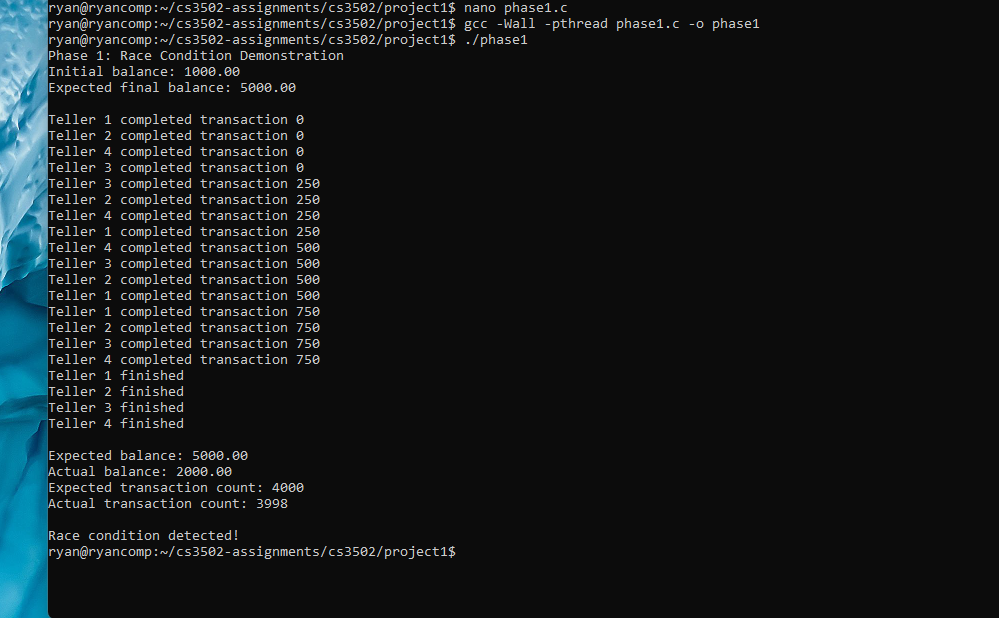
\includegraphics[width=\textwidth]{screenshots/phase1.png}
    \caption{Phase 1 showing an incorrect balance caused by a race condition.}
\end{figure}

\section{Phase 2: Mutex Protection}

For Phase 2, I added a pthread mutex to the account structure. Before changing the account balance or transaction count, each teller thread had to lock the mutex. After the update was finished, the thread unlocked it.

This made the account update a critical section. Only one teller thread could update the shared account data at a time.

After adding the mutex, the expected and actual balances were both 5000.00. The expected and actual transaction counts were also both 4000.

\begin{figure}[H]
    \centering
    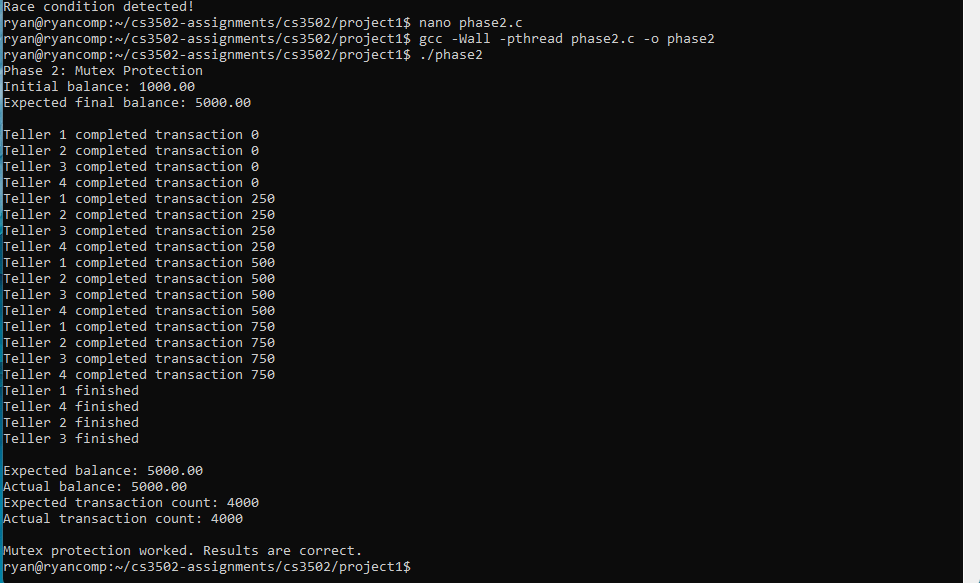
\includegraphics[width=\textwidth]{screenshots/phase2.png}
    \caption{Phase 2 showing the correct balance after adding mutex protection.}
\end{figure}

\section{Phase 3: Deadlock Creation}

In Phase 3, I created two accounts and two transfer threads. Thread 1 transferred money from Account 0 to Account 1. Thread 2 transferred money from Account 1 to Account 0.

Each thread first locked the account it was transferring money from. A delay was added before it tried to lock the second account. This made it likely that both threads would hold one lock at the same time.

Thread 1 held Account 0 and waited for Account 1. Thread 2 held Account 1 and waited for Account 0. Neither thread could continue, so the program entered deadlock.

I also added a monitor thread. After five seconds, it checked whether any transfers had completed. Since no transfer had completed, it printed a possible deadlock warning.

\begin{figure}[H]
    \centering
    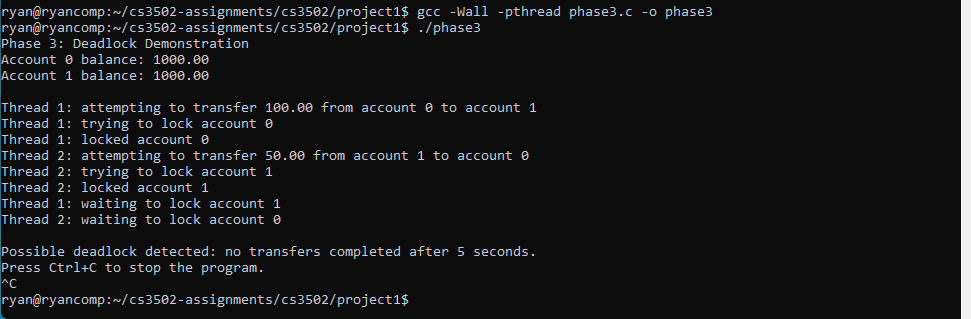
\includegraphics[width=\textwidth]{screenshots/phase3.png}
    \caption{Phase 3 showing both threads stuck and the deadlock warning.}
\end{figure}

\section{Phase 4: Deadlock Prevention}

For Phase 4, I fixed the deadlock using lock ordering. Every thread always locked the lower-numbered account first and the higher-numbered account second.

This meant both threads tried to lock Account 0 before Account 1, even when the transfer direction was reversed. One thread could wait for Account 0, but it would not hold Account 1 while waiting. This removed the circular wait condition.

Both transfers completed successfully. Account 0 ended with 950.00, Account 1 ended with 1050.00, and the total remained 2000.00.

\begin{figure}[H]
    \centering
    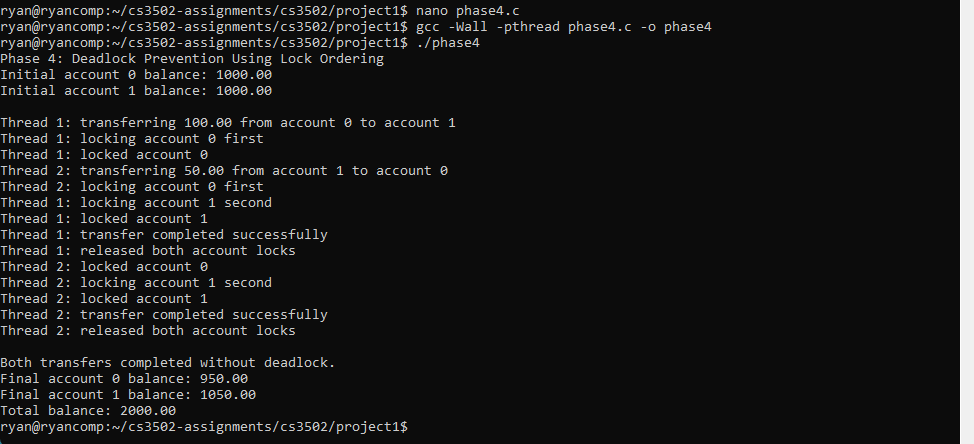
\includegraphics[width=\textwidth]{screenshots/phase4.png}
    \caption{Phase 4 completing both transfers without deadlock.}
\end{figure}

\section{Challenges and Solutions}

One challenge was making the race condition appear clearly. Without a delay, the race condition did not always produce an obvious incorrect result. I added a short usleep call between reading and writing the balance, which gave other threads time to access the same value.

Another challenge was making the deadlock happen reliably. I added a one-second delay after each thread locked its first account. This gave the other thread time to lock the opposite account.

The final challenge was stopping the deadlock. I solved this by using a consistent lock order based on the account numbers.

\section{Performance Observations}

Phase 1 completed in about 0.529 seconds. It did not have to wait for mutex locks, but it produced an incorrect final balance and transaction count.

Phase 2 completed in about 2.080 seconds. It took longer because each thread had to wait for the mutex before updating the account. Even though it was slower, the final balance and transaction count were correct.

Phase 3 did not complete because both threads became blocked forever.

Phase 4 also used mutex locks, but the transfers completed normally because the threads followed the same lock order.

\section{Conclusion}

This project showed why synchronization is important in multi-threaded programs. Without mutex protection, shared data can become incorrect. Using multiple locks without a plan can also create deadlock.

Mutexes fixed the race condition, and consistent lock ordering prevented the deadlock. The four phases demonstrated how a threaded program can first fail and then be corrected.

\end{document}
